%%%%%%%%%%%%%%%%%%%%%%%%%%%%%%%%%%%%%%%%%%%%%%%%%%%%%%%%%
\chapter[elua sur STM32F4-DISCOVERY]{elua sur STM32F4-DISCOVERY}
\label{chap:chap3}

\section{Qu'est-ce que Lua?}

Lua est un langage de script libre, réflexif et impératif. Il a été conçu afin de pouvoir être embarqué au sein d'autres applications et les étendre
Lua (qui signifie lune en portugais) a été développé par des membres du groupe de recherche TeCGraf, de l'université de Rio de Janeiro au Brésil.
Il est écrit en langage C ANSI strict, et grâce a cela il est compilable sur une grande variété de systèmes; le plus souvent est utilisé dans des systèmes 
embarqués, dont sa compacité est très appréciée, de plus, il possède la compatibilité du langage Cpour s'intégrer facilement dans la plupart des projets.
Il profite de la compatibilité que possède le langage C avec un grand nombre de langages pour s'intégrer facilement dans la plupart des projets. Lua a déjà
été utilisé pour le développement de jeux vidéo, entre eux, par exemple l'interface du jeu World of Warcraft de Blizzard Entertainment, SimCity4, entre 
autres.

\begin{figure}[h]
\begin{center}

\includegraphics[scale=0.4]{figure/eLua/Lua.JPG}
\caption{Logo Lua}
\end{center}
\end{figure}


\section{Qu'est-ce qu'eLua?}

  elua adopte le langage de programmation Lua pour faire une complète implémentation dans le monde de l'embarqué, elua ajoute des caractéristiques
spécifiques pour une efficacité, portabilité et développement de logiciels embarqués. eLua propose la totalité des caractéristiques de la version
de bureau de Lua, et c'est important de remarqué que elua utilise les mécanismes de base pour pouvoir l'étendre avec des fonctionnalités de développement 
de l'embarqué optimisés et spécifiques.
 

\begin{figure}[h]
\begin{center}
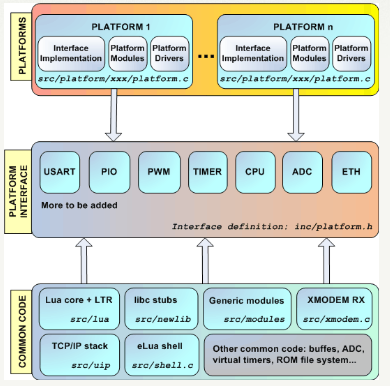
\includegraphics[scale=0.4]{figure/eLua/schema.png}
\caption{schema eLua}
\end{center}
\end{figure}

\section{Avantages de eLua}

\begin{description}

 \item[Contrôle total de la plateforme:] il n'existe pas un systèmee d'exploitation entre les programmes et le microcontrôleur.
 
 \item[Portabilité du code:] Comme Lua, le programme peut être executée dans un grand groupe varié de plateformes et architectures.

 \item[Facilité de transformation:] Le code et le design des produits pour eLua peuvent être conçu indépendament du matériel, ainsi toute changement ou
amélioration dans le future peut être fait facilement et gagner du temps.

 \item[Développement d'objectifs:] Lua est complètement fonctionnel avec la possibilité d'avoir un shell dans le microcontrôleur, il n'y a pas besoin 
de rien installer côté ordinateur a part la connexion du port ou ethernet. Les programmes sont utilisable directement dans les plateformes.

 \item[Flexibilité des produits:] 

Add modern high level script-language capabilities to your projects, resulting in highly adaptable, field-programable and reconfigurable designs. 
Efficient (and cheap!) future evolution to your systems.

\item[Shorter TTM:] Optimizes Time to Market, shorter time to revenue, improved ability to hit critical market windows, agility to survive in turbulent market conditions

    \item[Embedded RAD:] Prototype and experiment on a Rapid Aplication Develop model. Test your ideas directly on the target platforms and cheap development kits. No need for simulators or future code adaptations.

    \item[Ready to use kits:] A big (and growing) number of Open Source hardware and commercially available platforms are supported (see here ). Prototype cheap and fast and design your final hardware later using the produced code.

 \item[Long cycle de vie:]  Add user configuration and scripting capabilities to your projects, making them adaptable to the always changing contexts of industrial processes, evolving engineering, automation standards, field optimizations etc...


 \item[Apprendre l'embarqué: ] Simple interactive and interpreted experimenting cycle. Use your desktop programming skills to become an embedded systems developer in no time and with a lot of fun.

 \item[Open Source:] elua est libre, gratuit, et open source logiciel, comme Lua, elle possède une licence MIT qui permet l'utilisation de eLua dans des 
codes ``closed'' source. Il n'y a aucune permission a demander, ils demandent juste de faire circuler l'information au monde: on utilise eLua!
\end{description}


 

%What eLua is not?

 %   eLua is not an Operating System, although it offers some features and characteristics of one, like different File Systems, a command Shell, a remote console for Terminal access, ...

  %  eLua is not a stripped down set of Lua to fit in the embedded environment. Much on the contrary, it strives to offer the same features as the desktop version of Lua, complementing them with specific features for embedded use and discarting the need of an operating system running on the microcontrollers. Besides offering different flavors of the full Lua implementation (like the possibility of choosing between an integer-only and a floating point numbers implementation), a lot of work was and will be done in the direction of making Lua more "embedded-friendly" by augmenting the core language with features that allow lower memory requirements and faster embedded performance.

   % eLua is not a platform-specific development framework, much on the contrary. In eLua, you develop for a generic platform and run your Lua source code unchanged on a wide variety of platforms, offering the ancient dream of high level code portability among embedded platforms.

    %eLua is not an application for an OS or RTOS or a specific microcontroller.
    %eLua is self-contained, runs on "bare-metal" and has support for a large number of microcontroler architectures and models. For a list of the current supported platforms, please check our Status page.

   % eLua is not commercial software and there are no royalties or other charges for products based on it.

    %eLua is not GPL. Our legal MIT license, the same as Lua's, is more flexible and allows eLua to be incorporated in proprietary and commercially independent products.
